\documentclass[10pt]{article}
\usepackage[a4paper,margin=2.3cm]{geometry}
\usepackage[T1]{fontenc}
\usepackage{lmodern}
\usepackage{microtype}
\usepackage{amsmath}
\usepackage{booktabs}
\usepackage{graphicx}
\usepackage{xcolor}
\usepackage[hidelinks]{hyperref}
\usepackage[numbers,sort&compress]{natbib}
\usepackage{caption}
\captionsetup{font=small,labelfont=bf}
\graphicspath{{../figures/}{../reported/fp_analysis/}}
% Numbers quoted in the abstract; tables and text below use reported/curves/summary.json.
\newcommand{\PaperDice}{79.6}
\newcommand{\BratsReflectPooled}{81.7}
\newcommand{\BratsStrictMean}{64.1}
\newcommand{\BratsFA}{7.7}
\newcommand{\IxiFA}{29.0}
\newcommand{\IxiDiceOptDrop}{3.5}
\newcommand{\IxiMatchedDrop}{5.7}
\newcommand{\IxiAUPRC}{0.828}
\newcommand{\ThickAUPRC}{0.862}
\newcommand{\BratsAUPRC}{0.865}


\title{Healthy from where?\\[2pt]\large Evaluating a rectified-flow brain anomaly detector across protocols and hospitals}
\author{Matey Krastev\\\small Independent researcher \quad \texttt{matey.krastev@outlook.com}\\
\small Code and results: \url{https://github.com/m-krastev/brain-uad}}
\date{Technical report, October 2026}

\begin{document}
\maketitle

\begin{abstract}
Unsupervised anomaly detection (UAD) models for brain MRI learn what healthy anatomy looks like and flag what they cannot map back to it.
REFLECT (MICCAI 2025) does this with a rectified flow in the latent space of a medical VAE and reports state-of-the-art tumour segmentation on BraTS.
We reproduce REFLECT on BraTS 2021 T2 (pooled Dice \BratsReflectPooled{} against \PaperDice{} reported) and then evaluate it the way a deployed detector would be used: on all central slices of each test subject, including tumour-free ones, with the threshold fixed on validation subjects.
Under this protocol the mean Dice per tumour slice is \BratsStrictMean{}, and \BratsFA{}\% of tumour-free slices contain false positives, a quantity the original single-slice protocol cannot measure.
We then replace REFLECT's in-domain ``healthy'' training data, tumour-free slices of the BraTS patients themselves, with healthy volunteers scanned at other hospitals (IXI).
At each model's Dice-optimal threshold the cost looks small (\IxiDiceOptDrop{} points of pooled Dice), but false alarms rise from \BratsFA{}\% to \IxiFA{}\%; compared at a matched false-alarm budget the cost is \IxiMatchedDrop{} points of pooled Dice (first training seed; a second seed shows 38.8\% false alarms and a 10.5-point gap).
We test three remedies. Intensity harmonisation does not help. Simulated thick-slice acquisitions raise AUPRC from \IxiAUPRC{} to \ThickAUPRC{} for one training seed, but a second seed of plain IXI training reaches 0.879 (in-domain: \BratsAUPRC{}), so the gain is within seed variation; across these models a higher AUPRC went with more false alarms. Fine-tuning on tumour-free slices from 20--50 local subjects lowers false alarms and raises Dice at a matched false-alarm rate for both training seeds, while the same extra training without local data does not.
All comparisons come with paired subject-level bootstrap intervals, and the code, patches and per-slice results are public.
\end{abstract}

\section{Introduction}
Reconstruction-based UAD trains a generative model on healthy scans and scores each pixel by how much the model has to change it to make the scan look healthy \citep{baur2021autoencoders,lagogiannis2024deepdive}.
Diffusion models improved these reconstructions \citep{wyatt2022anoddpm,pinaya2022fast,behrendt2023pddpm}; REFLECT \citep{beizaee2025reflect} replaces iterative denoising with a rectified flow \citep{liu2023rectified} in the latent space of a VAE \citep{rombach2022ldm}, trained to transport synthetically corrupted slices back to their clean versions in a near-straight line, so that a single integration step yields the healthy counterpart.

Two parts of the standard evaluation make these results hard to carry over to a clinic.
First, the benchmark protocol scores one slice per test subject, the one with the largest tumour, and chooses the binarisation threshold on the test slices.
Tumour-free tissue in other slices never enters the score, so false alarms are invisible.
Second, the ``healthy'' training slices are tumour-free slices of the BraTS patients themselves: the same scanners, the same preprocessing, and the anatomy of tumour patients.
A hospital deploying UAD would instead train on healthy scans from elsewhere.
Both concerns have been raised for UAD in general \citep{meissen2022pitfalls,bercea2023aes,lagogiannis2024deepdive,reinke2024pitfalls}; here we quantify them for a current state-of-the-art method.

\paragraph{Contributions.}
(i) An independent reproduction of REFLECT on BraTS 2021 T2 from the authors' code, with the changes needed to run it on a single 16\,GB GPU.
(ii) A strict protocol (all 20 central slices, validation-fixed thresholds, a false-alarm rate on tumour-free slices) and a comparison at matched false-alarm budgets.
(iii) A cross-site experiment training on IXI healthy volunteers, an analysis of where the resulting false alarms occur, and three remedies: intensity harmonisation, thick-slice augmentation and local fine-tuning.
(iv) Paired subject-level bootstrap intervals for every comparison, repeated training seeds, and per-slice results from which all tables and figures can be recomputed on a CPU.

\section{Method and setup}
\paragraph{REFLECT.}
A frozen KL-f8 VAE pretrained on medical images encodes each $256\times256$ slice to a $4\times32\times32$ latent $z$.
A U-Net $v_\theta(z,t)$ is trained on healthy slices corrupted with synthetic anomalies to predict the straight-line velocity from the corrupted latent to the clean one.
At test time the latent is integrated for $K$ Euler steps ($K=5$ unless noted), decoded to a healthy reconstruction, and the anomaly map is the mean of the smoothed, clipped image-space and latent-space differences, exactly as in the released evaluation code.
We use the authors' code (commit \texttt{6e05909}) with a patch that loads the pickled VAE under PyTorch $\ge$\,2.6, encodes in chunks and splits each batch of 96 into micro-batches of 48 with size-weighted losses (identical gradients, as the U-Net uses GroupNorm only), and fixes the released test loader.
Training follows the paper: UNet-M, 200 epochs, batch 96, learning rate $5\times10^{-4}$.

\paragraph{Data.}
BraTS 2021 \citep{baid2021brats,menze2015brats,bakas2017tcga}: 1251 T2 scans with whole-tumour masks, split 80/10/10 by subject (seed 0).
From each scan we take the 20 central axial slices in SRI24 space \citep{rohlfing2010sri24}, map the brain's 1st--99th intensity percentiles to 0--255 and pad to 256.
Training and validation use tumour-free slices only.
IXI \citep{ixi}: 578 T2 scans of healthy volunteers from three London hospitals, skull-stripped with HD-BET \citep{isensee2019hdbet}, affinely registered to SRI24 with ANTs \citep{avants2011ants}, and sliced and scaled identically (7520 training slices).
IXI-trained models are trained for the same number of updates as the in-domain model.

\paragraph{Protocols.}
\emph{REFLECT protocol}: one slice per test subject (the largest tumour; 116 subjects), threshold swept on these test slices; we report the pooled Dice at the best threshold and the mean per-slice Dice at the best common threshold.
\emph{Strict protocol}: all 20 central slices of each of the 126 test subjects (2520 slices, 2144 with tumour, 376 tumour-free from 41 subjects), anomaly maps restricted to the brain mask, thresholds chosen on the validation subjects only.
We report pooled Dice, mean Dice over tumour slices, pixel-level AUPRC inside the brain, and the \emph{false-alarm rate}: the fraction of tumour-free slices with any positive pixel.
Thresholds are either Dice-optimal on validation, or the lowest threshold at which at most 5\% (or 10\%) of tumour-free validation slices fire.
Confidence intervals are 95\% percentile intervals from 2000 bootstrap resamples of test subjects \citep{efron1986bootstrap}, keeping all slices of a subject together and the validation thresholds fixed; differences between models use paired resamples.

\section{Results}
\subsection{Reproduction and the effect of the protocol}
Table~\ref{tab:protocol} and Fig.~\ref{fig:protocol} compare protocols for the model trained on tumour-free BraTS slices.
Under REFLECT's protocol our pooled Dice is 81.7 (80.8 with one step), against 79.6 reported; the mean per-slice Dice is 74.5.
The paper does not state which aggregate it reports, so the reproduction lies within this range.
Fixing the threshold on validation subjects instead of the test slices costs almost nothing (79.6 against a test-optimal 79.7).
Scoring all 20 central slices changes pooled Dice little, because large tumours dominate the pixel count, but the mean Dice over tumour slices falls to 64.1, and 7.7\% of tumour-free slices contain at least one false-positive pixel.

\begin{table}[t]
\centering\small
\caption{REFLECT on BraTS 2021 T2 (trained on tumour-free BraTS slices) under the original and strict protocols. Brackets: 95\% bootstrap intervals over test subjects.}
\label{tab:protocol}
\begin{tabular}{lll}
\toprule
Protocol & Dice & Notes \\
\midrule
Paper \citep{beizaee2025reflect}, REFLECT protocol & 79.6 & \\
Ours, REFLECT protocol, pooled & 81.7 & 1 step: 80.8 \\
Ours, REFLECT protocol, mean per slice & 74.5 & 1 step: 73.7 \\
Ours, strict, pooled & 79.6 [76.9, 81.9] & validation threshold \\
Ours, strict, mean over tumour slices & 64.1 [59.7, 68.3] & \\
\bottomrule
\end{tabular}
\end{table}

\begin{figure}[t]
\centering
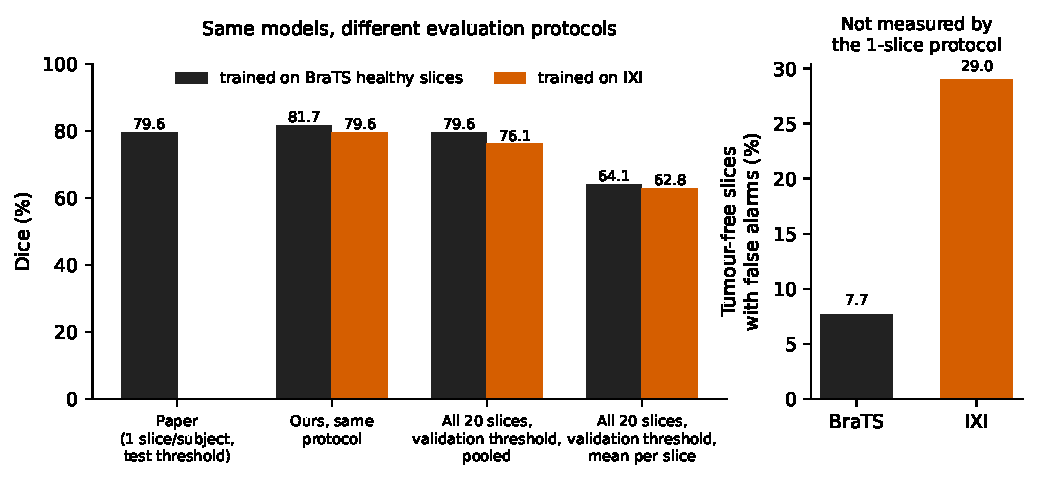
\includegraphics[width=\linewidth]{protocol.pdf}
\caption{Left: Dice of the BraTS-trained and IXI-trained models under four protocols. Right: false-alarm rate on tumour-free slices, which the single-slice protocol cannot measure.}
\label{fig:protocol}
\end{figure}

\subsection{Healthy training data from other hospitals}
Table~\ref{tab:site} reports all models on the strict protocol.
Replacing tumour-free BraTS slices with IXI healthy volunteers lowers AUPRC from 0.865 to 0.828 (paired difference $-3.8$ points, 95\% interval $[-5.7, -2.0]$) and pooled Dice at each model's Dice-optimal threshold by 3.5 points $[2.1, 5.0]$.
The same thresholds, however, let false alarms rise from 7.7\% to 29.0\% of tumour-free slices ($+21.3$ $[9.3, 35.3]$).
Each model thus reaches its best Dice at a different false-alarm rate, and comparing Dice-optimal scores understates the shift.
Comparing the models where each fires on 10\% of tumour-free test slices, the Dice gap is 5.7 points $[2.7, 12.3]$; at 5\% it is 11.6 points $[3.1, 25.4]$.
Fig.~\ref{fig:tradeoff} shows the full trade-off: the curves nearly meet at high false-alarm rates and separate at the low rates a screening tool would operate at.
Thresholds chosen on validation for a 5\% false-alarm rate gave 7--17\% on test, so validation false-alarm budgets transfer only roughly between subject sets.

\begin{table}[t]
\centering\small
\setlength{\tabcolsep}{4pt}
\caption{Strict protocol, 5 correction steps. FA: tumour-free test slices with any positive pixel (\%). ``10\% test FA'': threshold at which 10\% of tumour-free test slices fire, chosen per model and per bootstrap resample. Brackets: 95\% bootstrap intervals over the 126 test subjects. Paired differences are given in the text.}
\label{tab:site}
\begin{tabular}{lccccc}
\toprule
& & \multicolumn{2}{c}{Dice-optimal validation threshold} & \multicolumn{2}{c}{10\% test FA} \\
\cmidrule(lr){3-4}\cmidrule(lr){5-6}
Healthy training data & AUPRC & pooled Dice & FA & pooled Dice & mean Dice \\
\midrule
BraTS (in-domain) & 0.865 & 79.6 [76.9, 81.9] & 7.7 [2.5, 15.1] & 79.6 [76.8, 81.7] & 64.3 [59.5, 68.5] \\
IXI & 0.828 & 76.1 [72.6, 79.0] & 29.0 [17.2, 43.5] & 73.9 [66.3, 77.9] & 57.0 [47.8, 62.8] \\
IXI, thick-slice aug. & 0.862 & 77.7 [74.5, 80.5] & 42.3 [29.2, 57.2] & 67.6 [54.5, 75.6] & 49.1 [35.9, 59.1] \\
IXI, +10 ep.\ IXI only & 0.828 & 75.8 [72.5, 78.7] & 31.1 [19.3, 45.8] & 72.5 [66.1, 76.9] & 55.3 [48.6, 61.8] \\
IXI, +10 ep.\ 5 local & 0.829 & 76.4 [73.0, 79.1] & 27.7 [16.5, 41.8] & 73.0 [66.8, 77.3] & 55.6 [48.5, 61.7] \\
IXI, +10 ep.\ 20 local & 0.833 & 76.9 [73.8, 79.5] & 23.7 [14.0, 35.8] & 75.9 [71.9, 79.3] & 59.0 [54.0, 64.4] \\
IXI, +10 ep.\ 50 local & 0.834 & 76.8 [73.8, 79.3] & 22.9 [13.1, 35.0] & 76.3 [72.3, 79.3] & 60.4 [54.8, 65.2] \\
\bottomrule
\end{tabular}
\end{table}

\begin{figure}[t]
\centering
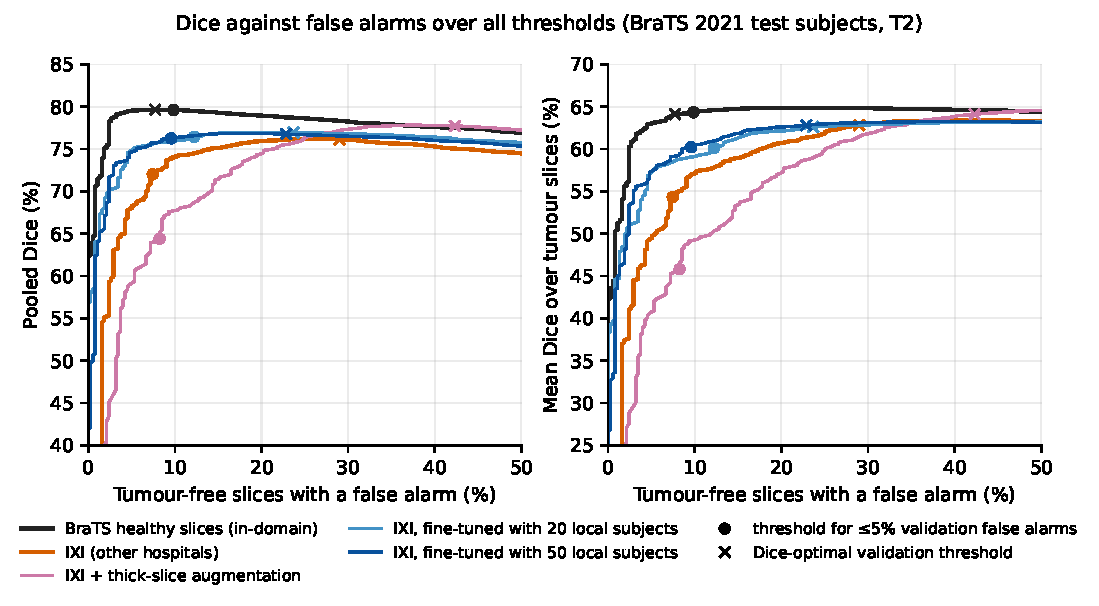
\includegraphics[width=\linewidth]{tradeoff.pdf}
\caption{Pooled Dice (left) and mean Dice over tumour slices (right) against the false-alarm rate on tumour-free test slices, over all thresholds. Crosses: Dice-optimal validation threshold; dots: threshold for at most 5\% validation false alarms.}
\label{fig:tradeoff}
\end{figure}

\subsection{Where the false alarms are}
On tumour-free test slices, the IXI model's false-positive pixels are bright (mean normalised intensity 0.45 against 0.27 for the brain), and only about 10\% lie within 8 pixels of the brain border, for both models.
A subject's false-alarm rate does not correlate with a through-plane sharpness proxy (Spearman $\rho=0.19$, $p=0.24$, 41 subjects), and 21.5\% of slices fire even in subjects whose 20 central slices contain no tumour, so neither slice thickness nor proximity to the tumour explains them.
Ventricle size and central CSF fraction show no significant correlation either, although IXI subjects have larger central CSF than BraTS subjects ($p<10^{-19}$).
Visually (Fig.~\ref{fig:qual} and the repository's \texttt{fp\_slices.png}), the flagged regions are ventricles enlarged or displaced by mass effect, low frontal slices near the skull base, and distorted anatomy.
The model trained on tumour-free slices of the BraTS patients reconstructs all of these.
We read this as anatomy leaking from patients into the in-domain ``healthy'' training data: those slices come from tumour patients whose brains are deformed by mass effect from the tumour elsewhere in the volume, which healthy volunteers do not show.

\begin{figure}[t]
\centering
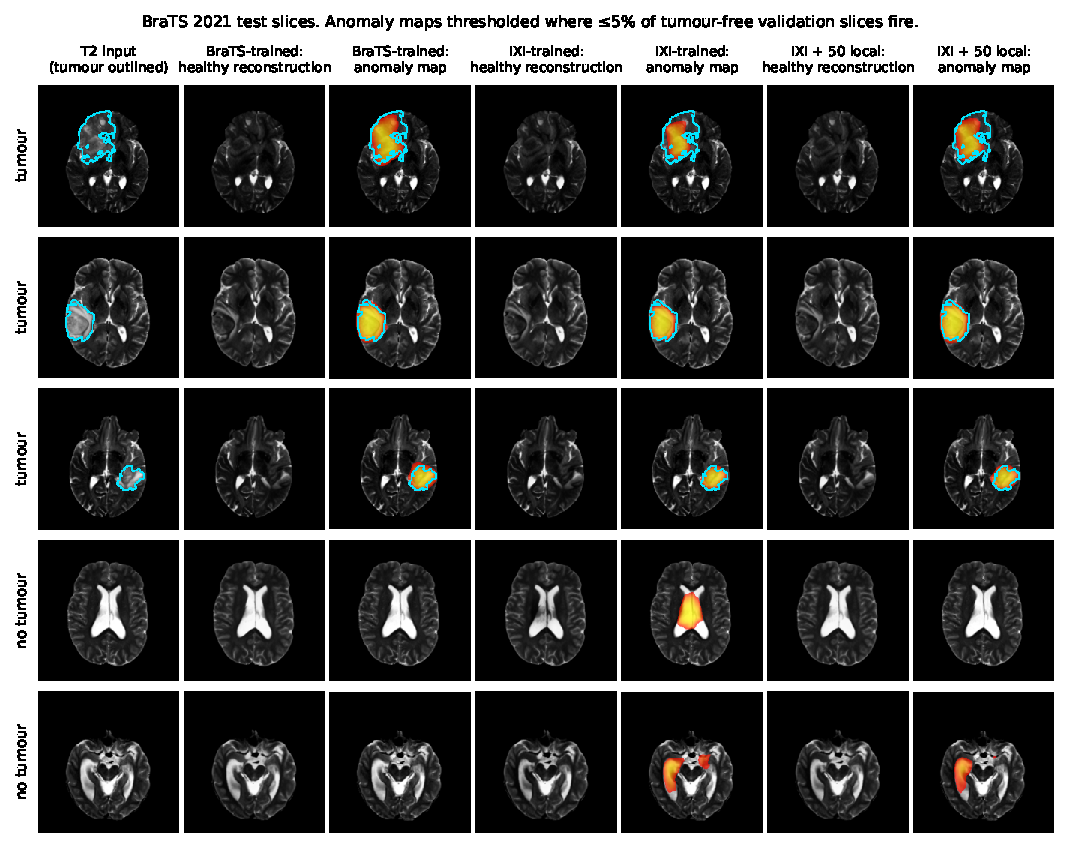
\includegraphics[width=\linewidth]{qualitative.pdf}
\caption{Test slices, healthy reconstructions and thresholded anomaly maps (threshold for at most 5\% validation false alarms; tumour outlined in cyan). Tumour rows are drawn at random from three size quantiles; the two tumour-free rows are the slices on which the IXI model fires most, chosen to show its failure mode.}
\label{fig:qual}
\end{figure}

\subsection{Remedies}
\paragraph{Intensity harmonisation.}
Matching each test subject's brain intensity histogram to the IXI training distribution before inference raises false alarms to 33.5\% and lowers pooled Dice to 75.0; the shift is not one of intensity distribution alone.

\paragraph{Thick-slice augmentation.}
Many BraTS T2 scans are thick-slice acquisitions resampled to 1\,mm.
We simulate this on IXI by averaging slabs of 1--6\,mm along a random axis and resampling.
AUPRC rises from 0.828 to 0.862 ($+3.4$ $[1.5, 5.5]$), nearly the in-domain 0.865, and Dice at the Dice-optimal threshold from 76.1 to 77.7.
The model also flags more healthy tissue, however: 42.3\% false alarms at that threshold, and at a threshold fixed for 5\% validation false alarms its pooled Dice is 64.4 against 72.0 for plain IXI training ($-7.6$ $[-9.2, -6.0]$) at similar test false-alarm rates (8.2\% and 7.4\%).
Threshold-free pixel metrics and Dice-optimal Dice can therefore favour a model that is worse at a clinically usable operating point.

\paragraph{Local fine-tuning.}
We continue training the IXI model for 10 epochs (learning rate $5\times10^{-5}$) on IXI plus the tumour-free slices of $N$ randomly chosen BraTS training subjects, oversampled ten times; $N=0$ is a control with the same extra training on IXI only.
Fig.~\ref{fig:local} shows paired differences from the IXI model.
With 20 and 50 local subjects, false alarms at the Dice-optimal threshold fall by 5.3 $[0.7, 10.1]$ and 6.1 $[1.6, 10.9]$ points, and pooled Dice at a 10\% test false-alarm rate rises by 2.0 $[0.6, 7.7]$ and 2.4 $[0.6, 7.9]$ points, recovering 35--42\% of the gap to the in-domain model.
The control changes neither (intervals include zero), so the gain comes from the local data, not from extra training.
Five local subjects are not enough.

\begin{figure}[t]
\centering
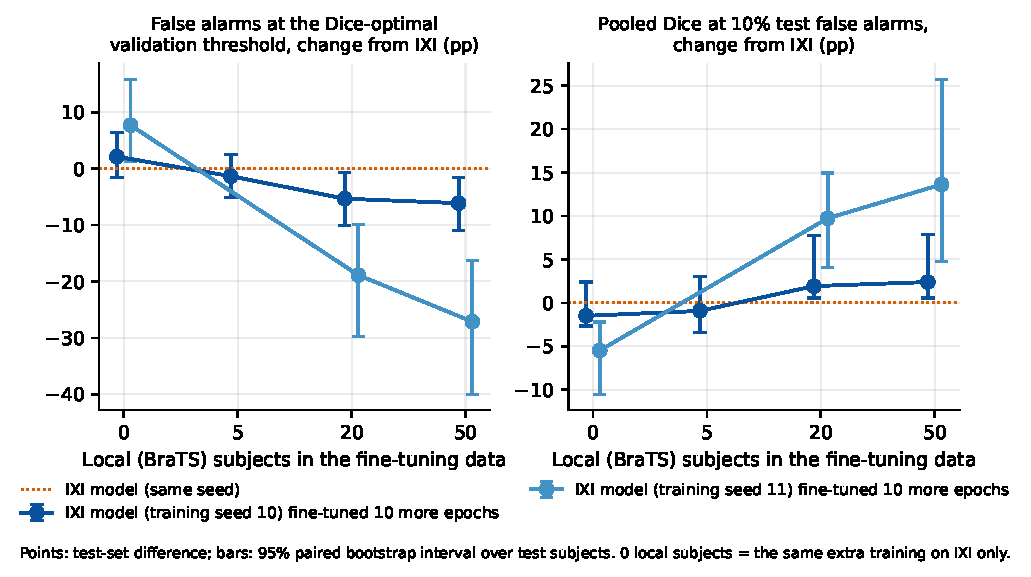
\includegraphics[width=0.85\linewidth]{local_finetuning.pdf}
\caption{Local fine-tuning: paired differences from the IXI model in false alarms at the Dice-optimal threshold (left) and in pooled Dice at a 10\% test false-alarm rate (right). Bars: 95\% paired bootstrap intervals. Dashed: the in-domain model.}
\label{fig:local}
\end{figure}


\section{Discussion}
REFLECT reproduces, and on its own benchmark it is as good as reported.
What changes under a deployment-like evaluation is the false-alarm rate on healthy tissue, which the single-slice protocol cannot measure and which Dice-optimal comparisons hide.
Two practical recommendations follow.
First, UAD methods should report a false-alarm rate on tumour-free slices and compare models at matched false-alarm budgets, or report the full Dice--false-alarm curve; AUPRC and best-threshold Dice can rank models in the wrong order, and should be repeated over training seeds.
Second, the usual in-domain training set, tumour-free slices of the patients themselves, is not ``healthy'' in the sense a deployment would need: it carries the patients' anatomy, including mass effect, into training.
Training on healthy volunteers from other hospitals exposes this, and a small amount of local data recovers part of the gap.

\paragraph{Limitations.}
We study one modality (T2), one dataset pair and 2D slices.
The tumour-free test set is small (376 slices from 41 subjects), so false-alarm rates have wide intervals and the correlation analyses are underpowered.
Bootstrap intervals cover the sampling of test subjects, not training randomness. A second training seed changed AUPRC by 5 points and false alarms by 10 points for the same IXI configuration, larger than some intervention effects, so single-seed comparisons of UAD methods should be read with care; the replicates of the thick-slice and in-domain models are reported in the repository as they complete.
No healthy scans from the BraTS sites exist, so our ``local'' fine-tuning data are tumour-free slices of other patients and inherit the anatomy leakage described above; a cleaner test would use a dataset with healthy controls and patients from the same scanners.

\paragraph{Reproducibility.}
All code, the patch to the authors' code, data splits, per-model JSON results and the per-slice threshold curves behind every table and figure are in the repository.
The evaluation of a model takes about four minutes on one 16\,GB GPU; everything after that (thresholds, intervals, figures) runs on a CPU in seconds.


\bibliographystyle{abbrvnat}
\bibliography{refs}
\end{document}
